\documentclass[10pt,a4paper]{article}
\usepackage[utf8]{inputenc}
\usepackage[english]{babel}
\usepackage[activate={true,nocompatibility},final,tracking=true,kerning=true,spacing=true]{microtype}
\usepackage[plainpages=false,pdfpagelabels,unicode]{hyperref}
\usepackage{fullpage}
\usepackage{graphicx}
\usepackage{fancyhdr}
\usepackage{occi}
\setlength{\headheight}{13pt}
\pagestyle{fancy}

%  just a test
% default sans-serif
\renewcommand{\familydefault}{\sfdefault}

% no lines for headers and footers
\renewcommand{\headrulewidth}{0pt}
\renewcommand{\footrulewidth}{0pt}

% header
\fancyhf{}
\lhead{GFD-R}
\rhead{\today}

% footer
\lfoot{occi-wg@ogf.org}
\rfoot{\thepage}

% paragraphs need some space...
\setlength{\parindent}{0pt}
\setlength{\parskip}{1ex plus 0.5ex minus 0.2ex}

%\renewcommand\paragraph{%
%  \@startsection{paragraph}{4}{0mm}%
%     {-\baselineskip}%
%     {.5\baselineskip}%
%     {\normalfont\normalsize\bfseries}}

% some space between header and text...
\headsep 13pt

\setcounter{secnumdepth}{4}

\begin{document}

% header on first page is different
\thispagestyle{empty}

Draft \hfill  Thijs Metsch, Intel\\
OCCI-WG \hfill  Mohamed Mohamed, Telecom SudParis\\
\rightline {\today}

\vspace*{0.5in}

\begin{Large}
\textbf{Open Cloud Computing Interface -- Platform}
\end{Large}

\vspace*{0.5in}

\underline{Status of this Document}

This document provides information to the community regarding the
specification of the Open Cloud Computing Interface. Distribution is
unlimited.


\underline{Copyright Notice}

Copyright \copyright ~Open Grid Forum (2014-2015). All Rights
Reserved.

\underline{Trademarks}

OCCI is a trademark of the Open Grid Forum.

\underline{Abstract}

This document, part of a document series, produced by the OCCI working
group within the Open Grid Forum (OGF), provides a high-level
definition of a Protocol and API. The document is based upon
previously gathered requirements and focuses on the scope of important
capabilities required to support modern service offerings.


\newpage
\tableofcontents
\newpage

\section{Introduction}
%!TEX root = nml-base.tex

\section{Introduction}%
\label{sec:introduction}

This document describes the base schema of the Network Markup Language (NML).
Section~\ref{sub:classes} defines the NML classes and their attributes and parameters.
Section~\ref{sub:relations} describes the relations defined between NML classes.

An NML network description can be expressed in XML\cite{xml}, and RDF/XML\cite{rdfxml} syntax.
Section~\ref{s:xmlschema} describes the XSD schema for the XML syntax.
Section~\ref{s:owlschema} describes the OWL 2 schema for the RDF/XML syntax.

These basic classes defined in this document may be extended, or sub-classed, 
to represent technology specific classes.

Section~\ref{s:examples} provides example use cases. This section is informative. 
Only sections~\ref{s:schema}, \ref{s:identifiers}, \ref{s:syntax}, and appendices \ref{s:xmlschema} and \ref{s:owlschema} are normative and considered 
part of the recommendation.

Appendix~\ref{s:g800terms} is informative and explains the relation between terms defined in this document and those defined in the ITU-T G.800 recommendation~\cite{g800}.

\subsection{Context}
\label{sec:context}

The Network Markup Language (NML) has been defined in the context of research and 
education networks to describe so-called hybrid network topologies. The NML is defined
as an abstract and generic model, so it can be applied for other network topologies as well.
See \cite{gfd.165} for an detailed overview including prior work.

\subsection{Scope}
\label{sec:scope}

The Network Markup Language is designed to create a functional description of 
multi-layer networks and multi-domain networks. An example of a multi-layered 
network can be a virtualised network, but also using different technologies. 
The multi-domain network descriptions can include aggregated or abstracted network topologies.
NML can not only describe a primarily static network topology, but also its potential capabilities (services) 
and its configuration.

NML is aimed at logical connection-oriented network topologies, more precisely topologies
where switching is performed on a label associated with a flow, such as a VLAN, wavelength or time slot. 
NML can also be used to describe physical networks or packet-oriented networks, 
although the current base schema does not contain classes or properties 
to explicitly deal with signal degradation, or complex routing tables.

NML only attempts to describe the data plane of a computer network, not the control 
plane. It does contain extension mechanism to easily tie it with network provisioning 
standards and with network monitoring standards.

Finally, this document omits a definition for the terms \emph{Network} or \emph{capacity}. 
This has been a conscious choice. The term \emph{Network} has become 
so widely used for so many diverse meanings that it is impossible to create a 
definition that everyone can agree on, while still expressing something useful.
See \emph{Topology} for the concept of a network domain and a \emph{Link} with multiple 
sources and sinks for the concept of a local area network.
The term \emph{capacity} is used by different technologies in such a different 
way (e.g.\ including or excluding the header and footer overhead) that it is better 
to let technology-specific extensions make an explicit definition.

\subsection{Notational Conventions}%
\label{sec:rfc2119}

The keywords “\MUST{}”, “\MUSTNOT{}”, “\REQUIRED{}”, “\SHALL{}”, “\SHALLNOT{}”, 
“\SHOULD{}”, “\SHOULDNOT{}”, “\RECOMMENDED{}”, “\MAY{}”,  and “\OPTIONAL{}” are 
to be interpreted as described in \cite{rfc2119}.
% except that the words do not appear in uppercase. 

This schema defines classes, attributes, relations, parameters and logic.
Objects are instances of classes, and the type of an object is a class.

Names of classes are capitalised and written in italics (e.g.\ the \emph{Node} class).
Names of relations are written in camel case and in italics (e.g.\ the \emph{hasNode} relation).
Names of identifiers and string literals are written in monspaces font (e.g. \texttt{Port\_X:in}).

Diagrams in this document follow the diagrammatic conventions of UML class diagrams.
\begin{itemize}
\item A subclass-superclass relationship is represented by a line with hollow triangle shape pointing to the superclass.
\item A whole-part relationship is represented by a line with a hollow diamond shape pointing to the whole (group).
\item A entity-relationship is represented by a line, optionally with numbers at each end indicating the cardinality of the relation. A named entity-relationship has a verb next to the line, and a filled triangle pointing to the object of the verb. (e.g. the entitity-relationship
\nmlrelation{BidirectionalPort}{*}{hasPort}{2}{Port} is named \emph{hasPort}, and each \emph{BidirectionalPort} is related to exactly 2 \emph{Port}s, and each \emph{Port} may be associated with zero, one or more \emph{BidirectionalPort}s.)
\end{itemize}



OCCI makes an ideal interoperable boundary interface between the web
and the internal resource management system of platform providers.

\section{Notational Conventions}
All these parts and the information within are mandatory for
implementors (unless otherwise specified). The key words "MUST", "MUST
NOT", "REQUIRED", "SHALL", "SHALL NOT", "SHOULD", "SHOULD NOT",
"RECOMMENDED", "MAY", and "OPTIONAL" in this document are to be
interpreted as described in RFC 2119 \cite{rfc2119}.


% begin platform content

\section{Platform}

The OCCI Platform document details how an OCCI implementation can model and implement a Platform as a Service API offering by extending the OCCI Core Model. This API enables the provisioning and management of PaaS resources. For example, it allows to deploy an application on one or more PaaS components. The application itself could be composed of different components. The main platform types defined within OCCI Platform are:

\begin{description}
  \item[Application] Which defines the user-defined part of the overall service.
  \item[Component] A configured instance of a piece of code providing business functions that are part of the execution of the application or responsible of hosting the application.
  \item[ComponentLink] Connects an \hl{Application} instance to a hosting \hl{Component} or connects two components.
\end{description}

\begin{figure}[!h]
	{\centering \resizebox*{0.7\columnwidth}{!}{\rotatebox{0}
	{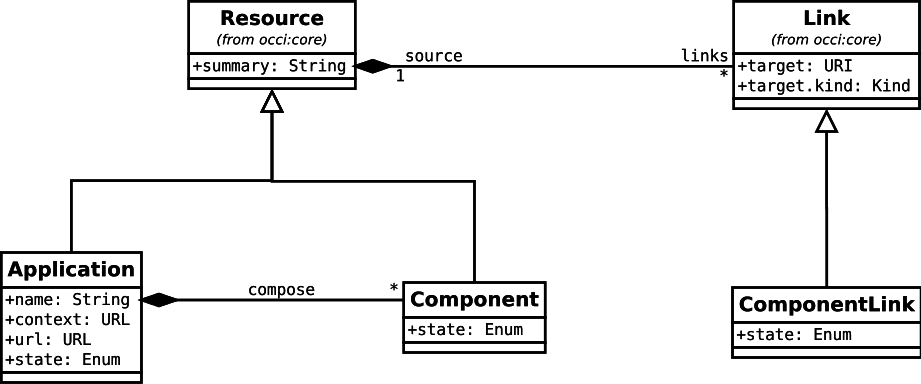
\includegraphics[scale=0.4]{figs/platform_overview.png}}} \par}
	\caption{Overview Diagram of OCCI Platform Types.}
	\label{fig:platform_uml}
\end{figure}

These platform types inherit the OCCI Core Model Resource base type and all their attributes. One can use a suitable transport protocol (e.g., HTTP) and a suitable rendering to discover and consume these resources. Independently of the implementation, the defined resources could be discoverable during runtime through OCCI compliant interfaces.

As required by the OCCI Core Model specification, every instantiated type that is a  sub-type of \hl{Resource} or \hl{Link} MUST be assigned a \hl{Kind} that identifies the instantiated type. Each such \hl{Kind} instance MUST be related to the Resource or Link base type's \hl{Kind}. That assigned \hl{Kind} instance MUST always remain immutable to any client.

\subsection{Application Kind Definition}
The following kind MUST be present and represents the kind definition of an application resource.

\hl{Application} inherits the \hl{Resource} base type defined in OCCI Core Model \cite{occi:core}. \hl{Application} is assigned the \hl{Kind} instance \textit{http://schemas.ogf.org/occi/platform\#application}. An \hl{Application} instance MUST use and expose this \hl{Kind}. The \hl{Kind} instance assigned to the \hl{Application} type MUST be related to the \textit{http://schemas.ogf.org/occi/core\#resource} \hl{Kind} by setting the \texttt{parent} attribute.

\mytablefloat{
	\label{tbl:app}\hl{Attribute}s defined for the \hl{Application} type.
}
{
	\begin{tabular}{lp{2.5cm}p{1cm}lp{5cm}}
	\toprule
	Attribute&Type&Multi\-plicity&Mutability&Description\\
	\colrule
	occi.app.name & String & 1 & Mutable & Name of the application.\\
	occi.app.context & URL & 1 & Immutable & URL for contextualizing the app.\\
	occi.app.url & URL & 1 & Immutable & DNS entry.\\
	occi.app.state & Enum \{active, inactive, error\} & 1 & Immutable & State of the application.\\
	occi.app.state.message & String & 0..1 & Immutable & Human-readable explanation of the current instance state.\\
	\botrule
	\end{tabular}
}

Table~\ref{tbl:app} describes the \hl{Attribute}s defined by an \hl{Application} instance. These attributes MAY or MUST be exposed by an instance of the \hl{Application} type depending on the ``Multiplicity'' column in the aforementioned table.

The \hl{Action}s are defined by the \hl{Kind} instance \textit{http://schemas.ogf.org/occi/platform\#application}. Every \hl{Action} instance in the table uses the \textit{http://schemas.ogf.org/occi/platform/application/action\#} categorisation scheme. ``Action Term'' below refers to \texttt{\hl{Action}.term}.

\mytablefloat{
	\label{tbl:app_actions}
	\hl{Action}s applicable to instances of the \hl{Application} type.
}
{
	\begin{tabular}{lll}
	\toprule
	Action Term & Target state & Attributes \\
	\colrule
	start & active & -- \\
	stop & inactive & -- \\
	\botrule
	\end{tabular}
}

The state model for the \hl{Application} instance is defined in Fig.~\ref{fig:app_state}.

\begin{figure}[!h]
	{\centering \resizebox*{0.5\columnwidth}{!}{\rotatebox{0}
	{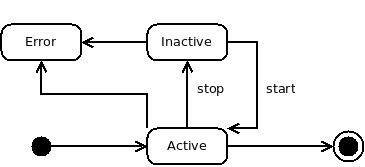
\includegraphics[scale=0.2]{figs/platform_component_state.png}}} \par}
	\caption{State model of an \hl{Application} instance.}
	\label{fig:app_state}
\end{figure}

\subsection{Component Kind Definition}
The following kind MUST be present and represents the kind definition of a component resource.

\hl{Component} inherits the \hl{Resource} base type defined in OCCI Core Model \cite{occi:core}. \hl{Component} is assigned the \hl{Kind} instance \textit{http://schemas.ogf.org/occi/platform\#component}. A \hl{Component} instance MUST use and expose this \hl{Kind}. The \hl{Kind} instance assigned to the \hl{Component} type MUST be related to the \textit{http://schemas.ogf.org/occi/core\#resource} \hl{Kind} by setting the \texttt{parent} attribute.

\mytablefloat{
	\label{tbl:component}\hl{Attribute}s defined for the \hl{Component} type.
}
{
	\begin{tabular}{lp{2.5cm}p{1cm}lp{5cm}}
	\toprule
	Attribute&Type&Multi\-plicity&Mutability&Description\\
	\colrule
	occi.component.state & Enum \{active, inactive, error\} & 1 & Immutable & State of the component.\\
	occi.component.state.message & String & 0..1 & Immutable & Human-readable explanation of the current instance state.\\
	\botrule
	\end{tabular}
}

Table~\ref{tbl:component} describes the \hl{Attribute}s defined by \hl{Component} instance. These attributes MAY or MUST be exposed by an instance of the \hl{Component} type depending on the ``Multiplicity'' column in the aforementioned table.

The \hl{Action}s are defined by the \hl{Kind} instance \textit{http://schemas.ogf.org/occi/platform\#component}. Every \hl{Action} instance in the table uses the \textit{http://schemas.ogf.org/occi/platform/component/action\#} categorisation scheme. ``Action Term'' below refers to \hl{Action}.{\tt term}

\mytablefloat{
	\label{tbl:component_actions}
	\hl{Action}s applicable to instances of the \hl{Application} type.
}
{
	\begin{tabular}{lll}
	\toprule
	Action Term & Target state & Attributes \\
	\colrule
	start & active & -- \\
	stop & inactive & -- \\
	\botrule
	\end{tabular}
}

The state model for the \hl{Component} instance is defined in Fig.~\ref{fig:component_state}.

\begin{figure}[!h]
	{\centering \resizebox*{0.5\columnwidth}{!}{\rotatebox{0}
	{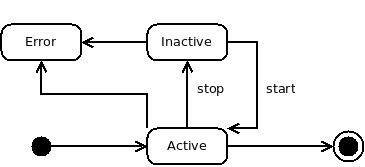
\includegraphics[scale=0.2]{figs/platform_component_state.png}}} \par}
	\caption{State model of a \hl{Component} instance.}
	\label{fig:component_state}
\end{figure}

\subsection{Linking to Components}

The composition of a service is realized through the linkage of \hl{Application} and \hl{Component} instances with each other.

\hl{ComponentLink} inherits the \hl{Link} base type defined in OCCI Core Model \cite{occi:core}. \hl{ComponentLink} is assigned the \hl{Kind} instance \textit{http://schemas.ogf.org/occi/platform\#componentlink}. The \hl{Kind} instance assigned to the \hl{ComponentLink} type MUST be related to the \textit{http://schemas.ogf.org/occi/core\#link} \hl{Kind} by setting the \texttt{parent} attribute.

The \hl{ComponentLink} kind can be further enhanced by the use of  provider-specific Mixins. This can be used to expose details such as database access URIs for an application linked up with a database component.

\subsection{Platform Templates}
Platform Templates allow for clients of an OCCI implementation to quickly and conveniently apply predefined configurations to OCCI Platform defined types. They are implemented using Mixin instances. There are two supported platform template types in OCCI Platform.

\subsubsection{Application Template}
Application templates allow clients to define which underlying framework the application should use (e.g., Programming language).

The Application Template is defined by a Mixin. A provider-specific defined Application Template Mixin MUST relate to the OCCI Application Template Mixin through the \texttt{depends} attribute in order to give absolute type information. The OCCI Application Template is defined by the \textit{http://schemas.ogf.org/occi/platform\#app\_tpl} Mixin and MUST be supported should Application Templates be offered.

Provider-specific Application Templates are constructed using a ``term'' and ``scheme'' combination where the ``term'' is a provider-specific description of the framework (e.g., python, ruby, \dots{}). Where an implementation requires additional information to be held in the Templates Mixin, it MAY do so by using \hl{Category}’s inherited \hl{Attribute}s.

\subsubsection{Resource Template}
The Resource Template Mixin builds upon the concept of Application Templates. A Resource Template is a provider defined Mixin instance that refers to a preset Resource configuration.

This can be used to define the resource instance attributes of the application and component. The provider-specific Resource Templates are defined by using a ``term'' and ``scheme'' combination. Those provider-specific Resource Template Mixin must relate to the OCCI Resource Template defined by \textit{http://schemas.ogf.org/occi/} \textit{platform\#res\_tpl} through the \texttt{depends} attribute. Where an implementation requires additional information to be held in the Templates Mixin, it MAY do so by using \hl{Category}'s inherited \hl{Attribute}s.

An example of these templates is shown in the following UML diagram in Figure~\ref{fig:templates}.

\begin{figure}[!h]
	{\centering \resizebox*{0.7\columnwidth}{!}{\rotatebox{0}
	{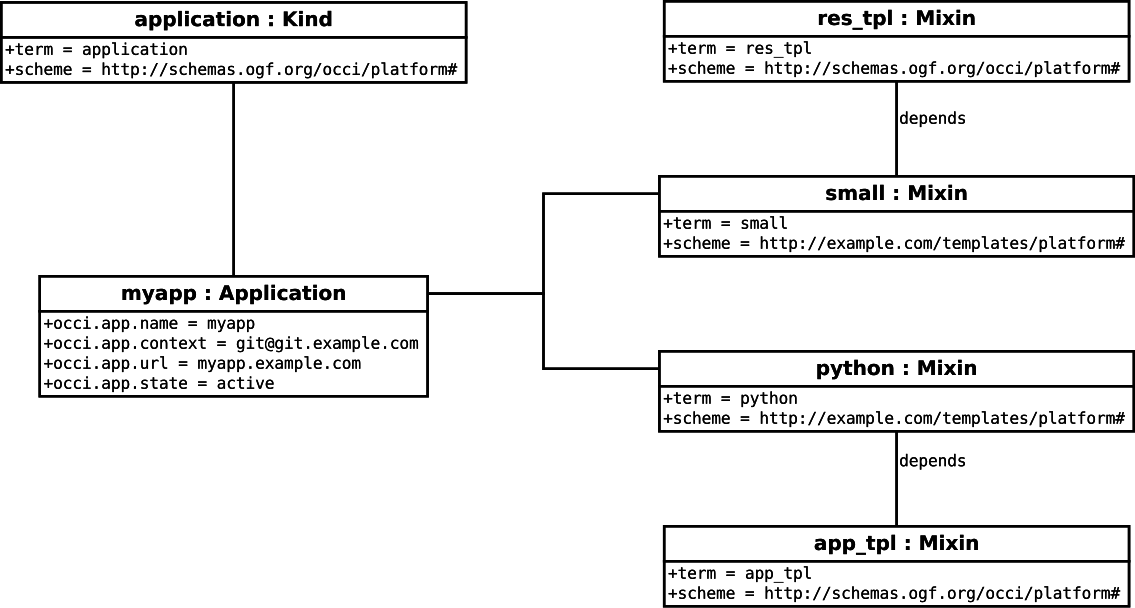
\includegraphics[scale=0.5]{figs/platform_templates.png}}} \par}
	\caption{Application and Resource Templates.}
	\label{fig:templates}
\end{figure}

\section{Specific Component Instance Mixins}
The following sections describe \hl{Mixin} instances, which SHOULD be implemented by Providers for some basic component type.

\subsection{Database Mixin}

\hl{Database} inherits the \hl{Mixin} base type defined in OCCI Core Model \cite{occi:core}. \hl{Database} is assigned the \hl{Mixin} instance \textit{http://schemas.ogf.org/occi/platform\#database}. The \hl{Database} instance \texttt{applies} to the \hl{Component} instance defined above.

\mytablefloat{
	\label{tbl:database}\hl{Attribute}s defined for the \hl{Database} type.
}
{
	\begin{tabular}{lp{2.5cm}p{1cm}lp{5cm}}
	\toprule
	Attribute&Type&Multi\-plicity&Mutability&Description\\
	\colrule
	occi.database.version & String & 1 & Immutable & Version of the database.\\
	\botrule
	\end{tabular}
}

Table~\ref{tbl:database} describes the \hl{Attribute}s defined by \hl{Database} instance.

\subsubsection{Database Link}
In case that an \hl{Application} instance links to a \hl{Component} instance, which has the \hl{Database} \hl{Mixin} instance applied the following \hl{Mixin} SHOULD be applied to the \hl{ComponentLink}.

\hl{DatabaseLink} inherits the \hl{Mixin} base type defined in OCCI Core Model \cite{occi:core}. \hl{DatabaseLink} is assigned the \hl{Mixin} instance \textit{http://schemas.ogf.org/occi/platform\#databaselink}. The \hl{DatabaseLink} instance \texttt{applies} to the \hl{ComponentLink} instance defined above.

\mytablefloat{
	\label{tbl:database_link}\hl{Attribute}s defined for the \hl{Database} type.
}
{
	\begin{tabular}{lp{2.5cm}p{1cm}lp{5cm}}
	\toprule
	Attribute&Type&Multi\-plicity&Mutability&Description\\
	\colrule
	occi.database.uri & URI & 1 & Immutable & Connection URI for the database instance.\\
	occi.database.username & URI & 0\ldots1 & Immutable & Username.\\
	occi.database.token & URI & 0\ldots1 & Immutable & Token.\\
	\botrule
	\end{tabular}
}

Table~\ref{tbl:database_link} describes the \hl{Attribute}s defined by \hl{DatabaseLink} instance.

% end platform content

\section{Security Considerations}
The OCCI Platform specification is an extension to the OCCI Core
Model specification \cite{occi:core}; thus the same security
considerations as for the OCCI Core Model specification apply
here.

\section{Glossary}
\label{sec:glossary}

\section{Glossary}
\label{s:glossary}

\begin{description}
\item[metric] a metric is a mathematical representation of a well defined aspect of a physical entity
\item[measurement] a measurement is the process of extracting a metric from a physical entity, and by extension also the result of such process. The measurement seldom corresponds exactly to the value of the metric.
\item[SLA] {\em ``An agreement defines a dynamically-established and dynamically
managed relationship between parties. The object of this
relationship is the delivery of a service by one of the parties within
the context of the agreement.''} from {\em SLA@SOI Glossary}
\item[Restful model] {\em ``REST is a coordinated set of architectural constraints that attempts to minimize latency and network communication, while at the same time maximizing
the independence and scalability of component implementations.''} \cite{fie02a}
\item[OCCI] {``\em The Open Cloud Computing Interface (OCCI) is a RESTful Protocol and API for all kinds of management tasks. OCCI was originally initiated to create a remote management API for IaaS model-based services, allowing for the development of interoperable tools for common tasks including deployment, autonomic scaling and monitoring''} \cite{occi:core}
\item[OCCI {\em Kind}] {\em''The Kind type represents the type identification mechanism for all Entity types present in the model''} \cite{occi:core}
\item[OCCI {\em \ln}] {\em''An instance of the Link type defines a base association between two Resource instances.''} \cite{occi:core}
\item[OCCI \mi] {\em''The Mixin type represent an extension mechanism, which allows new resource
capabilities to be added to resource instances both at creation-time and/or run-time.''} \cite{occi:core}
\item[OCCI \rs] {\em''A Resource is suitable to represent real world resources, e.g. virtual machines, networks, services, etc. through specialisation.''} \cite{occi:core}
\item[\sens] The \sens\ is a \rs\ that collects metrics from its input side, and delivers aggregated metrics from its output
\item[\coll] The \coll\ is a link that conveys metrics: it defines both the transport protocol and the conveyed metrics.
\end{description}


\section{Contributors}
We would like to thank the following people who contributed to this
document:

\begin{tabular}{l|p{2in}|p{2in}}
Name & Affiliation & Contact \\
\hline
Andy Edmonds & ICCLab, ZHAW & edmo at zhaw.ch \\
Peter Troeger & TU Chemnitz & peter@troeger.eu \\
Thijs Metsch & Intel & thijs.metsch@intel.com\\
Sami Yangui & & \\
Mohamed Mohamed & Telecom SudParis & \\
Philippe Merle & Inria & philippe.merle@inria.fr \\
\end{tabular}

Next to these individual contributions we value the contributions from
the OCCI working group.

\section{Intellectual Property Statement}
The OGF takes no position regarding the validity or scope of any
intellectual property or other rights that might be claimed to pertain
to the implementation or use of the technology described in this
document or the extent to which any license under such rights might or
might not be available; neither does it represent that it has made any
effort to identify any such rights. Copies of claims of rights made
available for publication and any assurances of licenses to be made
available, or the result of an attempt made to obtain a general
license or permission for the use of such proprietary rights by
implementers or users of this specification can be obtained from the
OGF Secretariat.

The OGF invites any interested party to bring to its attention any
copyrights, patents or patent applications, or other proprietary
rights which may cover technology that may be required to practice
this recommendation. Please address the information to the OGF
Executive Director.


\section{Disclaimer}
This document and the information contained herein is provided on an
``As Is'' basis and the OGF disclaims all warranties, express or
implied, including but not limited to any warranty that the use of the
information herein will not infringe any rights or any implied
warranties of merchantability or fitness for a particular purpose.


\section{Full Copyright Notice}
Copyright \copyright ~Open Grid Forum (2009-2011). All Rights Reserved.

This document and translations of it may be copied and furnished to
others, and derivative works that comment on or otherwise explain it
or assist in its implementation may be prepared, copied, published and
distributed, in whole or in part, without restriction of any kind,
provided that the above copyright notice and this paragraph are
included on all such copies and derivative works. However, this
document itself may not be modified in any way, such as by removing
the copyright notice or references to the OGF or other organizations,
except as needed for the purpose of developing Grid Recommendations in
which case the procedures for copyrights defined in the OGF Document
process must be followed, or as required to translate it into
languages other than English.

The limited permissions granted above are perpetual and will not be
revoked by the OGF or its successors or assignees.


\bibliographystyle{IEEEtran}
\bibliography{references}

\end{document}
